%% =====================================================================
%%  Part 2 --- draft v1
%%  Companion to "Revisiting Xia's Index of Substitution Saturation from
%%  a Mathematical Perspective" (Part 1, preprint).
%%
%%  Build:  pdflatex manuscript && pdflatex manuscript
%%  Figures: python Part_2/scripts/s41_figures.py
%% =====================================================================
\documentclass[preprint,12pt,authoryear]{elsarticle}

\usepackage[letterpaper,margin=1in]{geometry}
\usepackage{amsmath,amssymb,amsthm}
\usepackage{booktabs}
\usepackage{graphicx}
\usepackage{xcolor}
\usepackage{lineno}
\usepackage[hidelinks]{hyperref}

\setlength{\emergencystretch}{2em}

\newcommand{\Iss}{I_{ss}}
\newcommand{\Issc}{I_{ss.c}}
\newcommand{\Hbar}{\bar H}
\newcommand{\HFSS}{H_{FSS}}
\newcommand{\Issat}{I_{ss,\mathrm{sat}}}
\newcommand{\tr}{\operatorname{tr}}
\newcommand{\E}{\mathbb{E}}
\newcommand{\Var}{\operatorname{Var}}
\newcommand{\Cov}{\operatorname{Cov}}
\newcommand{\TL}{T_L}
\newcommand{\TLstar}{T_L^{*}}
\newcommand{\lam}[1]{\lambda_{#1}}

\newtheorem{theorem}{Theorem}
\newtheorem{lemma}[theorem]{Lemma}
\newtheorem{proposition}[theorem]{Proposition}
\newtheorem{corollary}[theorem]{Corollary}
\theoremstyle{definition}
\newtheorem{definition}[theorem]{Definition}
\theoremstyle{remark}
\newtheorem{remark}[theorem]{Remark}

\graphicspath{{figures/}}

\journal{Molecular Phylogenetics and Evolution}

\begin{document}
\linenumbers

\begin{frontmatter}

\title{Revisiting Xia's Index of Substitution Saturation, Part II:\\
       $\Issc$ is a power boundary, not a saturation threshold}

\author[dhu]{Zhi-Jie Xu\corref{cor1}}
\cortext[cor1]{Corresponding author.}

\address[dhu]{College of Biological Science \& Medical Engineering, Donghua
University, Shanghai 201620, China}

\begin{abstract}
We give an exact account of $\Issc$, Xia's critical value for substitution
saturation, and test it in a 20,000-fragment simulation.
$\Issc$ is used as a decision rule: when $\Iss$ exceeds $\Issc$, the data are
declared saturated and discarded. The rule cannot carry that weight.

For a four-taxon tree the critical tree is fixed by
$D(\TL)\sqrt L=z\sqrt{v_2(\TL)}$, with $D$ and $v_2$ exact sums
over the 256 site patterns. Three consequences follow, without simulation.
First, $\Issc$ does not measure the quantity that decides recoverability:
permuting taxa within columns preserves $\Iss$ exactly, to
$3\times10^{-15}$, while destroying the signal, and along that
family the recovery rate sweeps from $0.71$ to $1.00$ to $1/3$ with $\Iss$
fixed. Second, the length dependence is not a power law with a universal
exponent; it is $\lam{\Iss}/(2\lam D-\lam{v_2})$, a ratio of two local
rates that ranges from $0.061$ to $0.585$ across configurations. Third, for a
subset of a concatenation it is unreliable for the decision asked of it.

Running through all three is an identity: $D$ is exactly the
Kullback--Leibler distance from the tree to its own best star approximation.
The Farris zone is therefore not a separate mechanism but the region where
that distance is smallest; over a controlled family $D$ moves by a factor of $3583$
while $\Iss$ moves by $2.6\%$. In the local limit the boundary reduces to one
number: $\Issc(L)$ is the index of the tree whose KL distance to its own best
star approximation is $5.41/L$.

At genome scale the account is tested. Resampled $500$ bp fragments from one
$16$-taxon tree, banded by $\Iss$ at thresholds measured on that same tree,
reconstruct it exactly once concatenated to $10$ kbp; above $100$ kbp no band differs from any other. The
threshold sits where recovery has fallen six points from its peak.
\end{abstract}

\begin{keyword}
substitution saturation \sep index of substitution saturation \sep
statistical power \sep partition filtering \sep quartet \sep
phylogenetic signal
\end{keyword}

\end{frontmatter}

%% =====================================================================
\section{Introduction}

\citet{xia2003iss} introduced the index of substitution saturation $\Iss$
and its critical value $\Issc$, tabulated by sequence length and number of
taxa. Part~I \citep{xu2026preprint} showed that $\Iss$ is an
average over sites and
cannot depend on $L$ except through finite-sample noise, so
$\Var(\Iss)=\Theta(L^{-1})$ exactly and the critical value must move with
$L$ to hold a decision level fixed.

That leaves open what $\Issc$ \emph{is}. It is a number that moves with $L$,
on a scale whose ceiling depends on the entropy convention; it is used as a
discard rule; and, as we show here, it does not measure the thing that
determines whether a topology can be recovered.

The paper is organised around three constructions, all exact and all
reproducible from the accompanying scripts: a family of data sets with
identical $\Iss$ whose recovery rates span the whole possible range
(\S\ref{sec:shuffle}); matched-$\Iss$ genuine trees whose recovery differs by
up to $125$-fold (\S\ref{sec:matched}); and an exact decomposition of the
length exponent into two measurable rates, with a one-factor-at-a-time
account of which tree geometry moves which rate (\S\ref{sec:factors-results}).

Section~\ref{sec:subset} states the practical consequence first, because it
follows from the definition of the criterion rather than from any of the
machinery that follows, and it governs how the index should be used.

One result deserves flagging before the machinery, because it reorganises the
subject. The Farris zone and the length dependence of $\Issc$ are usually
discussed separately --- one as a property of trees, the other as a property
of the index, and in different literatures. They are the same quantity seen
twice. The per-site gap $D$ that sets the critical tree is, exactly, the
Kullback--Leibler distance from the tree to its best star approximation; the
Farris zone is the region of tree space where that distance is smallest.
Section~\ref{sec:shared} establishes this and quantifies it, and it is why
the factor that dominates the length exponent (\S\ref{sec:factors-results}) is the
same one that dominates the zone.

\paragraph{Where this sits.} Two literatures are adjacent to this question
and neither has this object. One critiques $\Iss$ and its relatives on the
ground of model violation --- non-homogeneity, compositional heterogeneity,
the treatment of invariant sites --- and responds by building better
statistics and calibrating them by simulation
\citep{jermiin2020signal,duchene2022saturation}. Those critiques are
\emph{conditional}: their common form is that the index fails when the model
is wrong. The other derives closed forms for experimental design --- how much
data a quartet needs, what substitution rate is optimal --- without ever
acting on a diagnostic statistic. \citet{townsend2007} derives the optimal
rate for a dated four-taxon polytomy, which is to say a star, and
\citet{townsend2012} extend that to a signal-and-noise decomposition of a data
set's power to resolve a phylogeny. The gap this paper occupies is the join:
the analytic objects of the second literature applied to a statistic of the
first.

The claim made here is correspondingly \emph{structural} rather than
conditional. The index fails to measure what its name says even when the
model is exactly right and the usage exactly as prescribed:
\S\ref{sec:shared} exhibits two configurations whose per-branch
multiple-substitution profile is identical to the last digit and whose
$D$ differs by a factor of $36$. No accumulation of conditional
criticisms yields that statement, and it does not depend on any of their
conditions.

Positioning that connection is worth one paragraph, because it places the
paper in a debate it would otherwise appear to be ignoring. The Farris zone
was named by \citet{siddall1998} for the four-taxon case in which the long
branches are sisters, parsimony recovers the tree and likelihood does not ---
as against the zone of \citet{felsenstein1978}, where the long branches are
separated and parsimony itself is inconsistent. The two are not symmetric in
kind: the first is a statement about consistency and holds however much data
are supplied, the second is a statement about power and dissolves as data
accumulate. That asymmetry is what makes the Farris zone's boundary
length-dependent, and it is the reason \citet{leuchtenberger2020} call the
zone ``not unambiguously defined for ML inference'' and simulate the whole
branch-length plane instead of locating a boundary. Equation
\eqref{eq:resolution} is that boundary. The argument of
\citet{swofford2001} against \citet{siddall1998} --- that parsimony succeeds
there through its own bias rather than because likelihood is repelled --- is
therefore the same claim as ours in prose; what is new here is the closed
form, and with it the demonstration that the moving threshold in Xia's tables
is that boundary and not a saturation threshold at all.

The paper closes on that boundary at a scale where it can be spent.
\S\ref{sec:genome} bands twenty thousand resampled short fragments by $\Iss$
and asks whether the band a filter would discard is in fact unusable, and
whether a method immune to long-branch repulsion benefits from the filter;
the answers are no and no, and the second answer has a mechanism that
\S\ref{sec:w3} computes exactly. Throughout, $\Issc$ is defined by our own
resampling on our own tree, and the tabulated values are used only as a
statement about which factors matter.

%% =====================================================================
\section{Methods}
\label{sec:methods}

%% =====================================================================
\subsection{Three topologies, three likelihoods, exactly}
\label{sec:quartet}

A quartet has three candidate topologies and therefore three likelihood
functions. Each is a sum of $L$ independent per-site terms, so
$(\ell_1,\ell_2,\ell_3)$ is jointly asymptotically normal and
\begin{equation}
\Pr[\text{correct}]=\Pr[\ell_1>\ell_2\ \wedge\ \ell_1>\ell_3]
\end{equation}
is a bivariate normal orthant probability whose means, variances and
correlation are sums over the 256 site patterns. No simulation is required
and no closed-form branch-length maximum-likelihood estimate is needed ---
none exists.

\begin{lemma}[Star projection]
\label{lem:star}
Both wrong topologies of a quartet have the same Kullback--Leibler projection,
the \emph{star}: at zero internal branch the tree is the same regardless of
which split it claims, and the star family is described identically in all
three parametrisations.
\end{lemma}

\begin{remark}
The lemma is checked rather than assumed. Scanning $219$ configurations by
objective rather than by fitted branch length, the largest relative KL gain
over the star anywhere is $2.5\times10^{-6}$; see \S\ref{sec:notes}.
\end{remark}

\begin{proposition}[Two-way reduction]
\label{prop:two-way}
Under Lemma~\ref{lem:star} the three-way choice reduces \emph{exactly} to a
two-way one, and
\begin{equation}
\Pr[\text{correct}]=\Phi\!\left(\frac{\sqrt L\,D}{\sigma}\right),
\label{eq:two-way}
\end{equation}
with $D$ the per-site KL gap to the better alternative.
\end{proposition}

\begin{proof}
The two wrong fits coincide, so $\ell_2=\ell_3$ identically and
$\Pr[\ell_1>\ell_2\wedge\ell_1>\ell_3]=\Pr[\ell_1>\ell_2]$. That is a
one-sided normal probability with mean $\sqrt L\,D$ and standard
deviation $\sigma$.
\end{proof}

One degenerate corner must be handled separately, and only a construction
whose purpose is to remove all signal reaches it: when the three \emph{fitted}
distributions coincide, all three likelihoods are one number and the answer is
$1/3$, not $\Phi(0)=1/2$. See \S\ref{sec:notes}.

%% =====================================================================
%% =====================================================================
\subsection{The critical tree}
\label{sec:factors}

Define $\Issc(L)$ by resampling: the $\Iss$ of the tree at which the recovery
rate reaches $95\%$. This is a definition rather than a fit, needs no
external data, and makes the question one of internal consistency.


\begin{theorem}[Resolution condition]
\label{thm:resolution}
Let $D$ be the per-site Kullback--Leibler gap between the true tree and
the better of the two alternatives, and $v_2$ its per-site variance. The tree
length at which the recovery probability falls to the level $z$ of a
one-sided test, $z=\Phi^{-1}(1-\alpha)$, satisfies
\begin{equation}
D(\TL)\,\sqrt L \;=\; z\,\sqrt{v_2(\TL)} .
\label{eq:resolution}
\end{equation}
\end{theorem}

\begin{proof}
By \eqref{eq:two-way} the recovery probability is
$\Phi(\sqrt L\,D/\sigma)$, so the level is reached when
$\sqrt L\,D/\sigma=z$. The denominator is
$\sigma^2=v_2$ by definition, which gives \eqref{eq:resolution}.
\end{proof}

\begin{corollary}[Exponent of the length dependence]
\label{cor:exponent}
Writing $\lam{\bullet}$ for the local log-derivative with respect to the tree
scale, the critical tree and the index at it satisfy
\begin{equation}
\frac{\mathrm d\log \TLstar}{\mathrm d\log L}
=\frac{1}{2\lam D-\lam{v_2}},
\qquad
\Issc(L)=\Issat-C\,L^{-p},
\qquad
p=\frac{\lam{\Iss}}{2\lam D-\lam{v_2}} .
\label{eq:exponent}
\end{equation}
\end{corollary}

\begin{proof}
Differentiate \eqref{eq:resolution} with respect to $\log L$. With
$r=\mathrm d\log\TLstar/\mathrm d\log L$, the left side contributes
$\sqrt L\,(\lam D\,r+\tfrac12)$ and the right side
$D\sqrt L\,\tfrac12\lam{v_2}\,r$, using $z\sqrt{v_2}=D\sqrt L$ from
\eqref{eq:resolution} itself. Equating them gives
$r(\lam D-\tfrac12\lam{v_2})=-\tfrac12$, that is the first relation. The
index at the critical tree then moves as
$\mathrm d\log\Issc/\mathrm d\log L=\lam{\Iss}\,r$, which is the third, and
integrating gives the second.
\end{proof}

The exponent is therefore a ratio of two independently measurable rates:
$\lam{\Iss}$ is how fast $\Iss$ saturates with tree length, and $\lam D$
is how fast the topological signal decays --- that is, the multiple-hit effect
itself.


%% =====================================================================
\subsection{The simulation experiment}
\label{sec:design}

The exact results need no simulation; the genome-scale test does, and its
design is fixed before any measurement is taken.

The tree is a single $16$-taxon Yule--Harding tree drawn once by AliSim and
kept for the whole study. Fragments are $500$~bp simulated under that tree
with every branch length multiplied by a common scale $s$, for twenty values
of $s$ spanning $0.04$ to $6$, so that tree length is the only parameter that
varies and the topology is held fixed. Twenty thousand fragments are drawn
this way, forming a pool of $10$~Mbp. Because sites are i.i.d., a long
alignment chopped into $500$~bp pieces is exactly a set of independent
$500$~bp fragments, so one AliSim call per scale produces a whole block of
the pool.

$\Iss$ is computed per fragment, convention~A, from the simulated bases.
The two thresholds that partition the pool are then measured on this same
tree by the resampling procedure of \S\ref{sec:factors}: a fragment is
called clean by a length-$L$ calibration when its $\Iss$ lies below
$\Issc(L)$. The arms are the bands between the thresholds, plus the
integrated pool; each is truncated to the same number of sites, so that the
arms differ only in composition and not in length.

Three methods are run on every arm: maximum likelihood under JC69 through
IQ-TREE, and both CASTER variants. Recovery is scored as the
Robinson--Foulds distance to the true tree, whose maximum on $16$ taxa is
$26$. Uncertainty is estimated by a delete-a-block jackknife over the
fragment pool rather than by independent replicates, because the question is
how the result depends on which fragments were drawn; the pool is split into
ten consecutive blocks and each is deleted in turn.

%% =====================================================================
\subsection{Software and reproducibility}
\label{sec:software}

Simulation uses AliSim and recovery uses IQ-TREE; \texttt{caster-site} and
\texttt{caster-pair} are used unmodified. The quartet results --- the
resolution condition, the exponent decomposition, the orthant probabilities
and the closed form for CASTER's score --- are computed by enumeration and
orthant quadrature and need no external binary at all.

Every number in this paper is produced by a script in the archive, one per
result set, and every table is read from the CSV that script writes. Code
and result tables are at
\url{https://github.com/Gipsy-The-Sheller/Iss_simulations}, which holds both
papers of this series; the tag \texttt{rs-preprint} is the version this
manuscript was built from.

%% =====================================================================
\section{Results}
\label{sec:results}

%% =====================================================================
\subsection{The criterion is not valid for a subset of a concatenation}
\label{sec:subset}

Substitution saturation is a property of the substitution process. A
subsample of an alignment underwent the same process as the whole: it is a
window onto the same history, not a different history. Any quantity that
measures saturation --- the frequency of multiple hits, the fraction of sites
made homoplastic, the expected site entropy --- has the same expectation on
the subsample as on the whole.

An alignment of $10{,}000$~bp may have $\Iss<\Issc$ while a $500$~bp
subalignment of it has $\Iss>\Issc$. This is not evidence that the subsample
is more saturated. It is two effects, neither of them saturation.

\begin{enumerate}
\item $\Iss$ is a per-site average, so $\E[\Iss]$ is the same for any subset
  of sites; the difference between the two observed values is estimator
  noise, with standard error $\Theta(L^{-1/2})$, four and a half times larger
  at $L=500$ than at $L=10{,}000$.
\item $\Issc(L)$ \emph{increases} with $L$ (\S\ref{sec:factors}). The
  threshold at $L=500$ is lower than at $L=10{,}000$, so the same data cross
  it more easily. The data did not change; the threshold did.
\end{enumerate}

Therefore:

\begin{enumerate}
\item[(i)] $\Issc$ has a defined decision-theoretic meaning only for the
  whole data set it was computed for. Applied to a partition, a gene, a
  single-copy locus, or any subalignment, the comparison $\Iss>\Issc$ no
  longer tests the hypothesis it names, and the resulting decision --- in
  particular the decision to \emph{discard} a partition as saturated --- is
  not supported by the statistic.
\item[(ii)] The power of the criterion is a property of the full set. A
  subset has less power by construction, and no reading of $\Iss>\Issc$ on a
  subset recovers it.
\item[(iii)] Consequently the operative question for a partition is not its
  saturation level but whether it carries a different history --- the
  evolutionary-heterogeneity question. Saturation is a shared property of the
  whole alignment's substitution process; heterogeneity is not, and it is the
  one that partitioning actually addresses.
\item[(iv)] Where a method can down-weight rather than exclude, it dominates
  discarding. Quartet-based and supertree methods admit exactly this:
  weighted ASTRAL \citep{zhang2018} assigns each gene tree a quantitative
  weight, so an unreliable or conflicting partition contributes less without
  being thrown away, and the information it does carry is retained. A binary
  discard/keep rule based on $\Issc$ cannot express that, and the replacement
  of a graded weight by a threshold is a loss of information that no choice
  of threshold recovers. The empirical literature on the practice this
  replaces --- \citet{duchene2022saturation} is the most direct recent
  example --- measures how much is lost by excluding loci, and the question
  is quantitative rather than binary in exactly that way.
\end{enumerate}

This is not a hypothetical. Slicing an alignment into blocks and judging each
block against the threshold tabulated for the block's length gives a
quantitative version (Fig.~\ref{fig:domain}). The blocks are slices of the
same alignment, so their expected $\Iss$ is the whole's --- that is, exactly
the whole's threshold. The threshold they would be judged against, however,
is the one tabulated for the shorter length, and it is lower. Across four
$(\text{block},\text{whole})$ pairs, spanning whole lengths from $4000$ to
$40{,}000$, the block's mean sits $2.3$ to $3.0$ block standard deviations
above its own threshold, and between $19.8$ and $20.0$ of every $20$ blocks
are declared saturated while the whole passes.

Below some alignment length the criterion is not merely wrong but undefined.
For the Farris tree of Fig.~\ref{fig:flat} no tree length reaches a $95\%$
recovery rate at any $L\le10^4$ --- at $L=3000$ the best achievable rate over
all tree scales is $0.755$ --- so there is no threshold to compare against.
A tabulated $\Issc$ supplies a number at every length regardless, so in
practice a verdict is always available; it is simply not a verdict the data
support.

A corollary, stated carefully, because the obvious version of it is wrong.
If the failure were caused by saturation, discarding sites would look
rational, since more data could not help. If it is caused by power, the
tempting conclusion is that discarding is backwards --- deleting data to cure
a shortage of data. That conclusion does not follow, and an earlier draft of
this section drew it. What matters is not how many sites are removed but
whether the removed ones carried signal. Filtering on site entropy --- which
is what the index does, one site at a time --- keeps the informative sites
and drops the rest, and in this framework it \emph{helps}: measured on three
configurations at their critical trees, removing the sites above entropy
$0.90$ raises standardised signal by $22\%$, $40\%$ and $337\%$. The practice
of discarding saturated sites is therefore not refuted by the power reading.

What the power reading does say is narrower and survives: the benefit is a
property of \emph{which} sites the filter selects and not of how many, so it
is not transportable. A filter calibrated on one configuration selects a
different set of sites on another, and \S\ref{sec:shared} shows the index
varies enough between configurations to make that the dominant consideration
--- at a fixed alignment length, the same index reads $0.33$ on one tree and
$0.99$ on another. The remedy is not "keep the data" or "discard the data"
but "know which sites your filter is removing", and that is a question about
the configuration rather than about the index.

Finally, the correlation that makes the rule look reasonable in practice is a
confounding. Short partitions often are fast-evolving genes --- third codon
positions, rRNA loop regions --- and it is the rate, not the length, that
saturates them. That is precisely why the question of \S\ref{sec:subset}(iii)
is the right one to substitute.

%% =====================================================================
%% =====================================================================
\subsection{$\Iss$ does not determine recoverability}
\label{sec:shuffle}

\paragraph{Relation to Part~I.} Part~I
\citep{xu2026preprint} already reports that along a four-taxon transfer of
long branches at fixed patristic total, the index is constant while recovery
spans its full range, and that a fifteen-fold change in the tree length at
which recovery fails moves the index by $1.2\%$. Those are the same
phenomena studied here, and the present section is a strengthening rather
than a discovery: Part~I's invariance holds along a path that
preserves the patristic total, whereas the construction below holds $\Iss$
fixed \emph{exactly}, to machine precision, at every point of a family that
is not a path of trees at all. What is new in Part 2 is the mechanism
\eqref{eq:resolution}, the exponent decomposition, the identity
\eqref{eq:delta-is-kl}, and the consequences of \S\ref{sec:subset}; what is
not new is the observation that the index fails to track recoverability.

\begin{proposition}[Invariance under within-column permutation]
\label{prop:shuffle}
Permute the taxa \emph{within each column}, independently per column, and let
$P_f=(1-f)P+fQ$ where $Q$ is the average of $P$ over all $24$ relabellings.
Then $\Iss(P_f)=\Iss(P)$ exactly, for every $f\in[0,1]$.
\end{proposition}

\begin{proof}
Each column keeps its multiset of bases, so the site entropy $h$ is unchanged;
each column contributes the same counts to the pooled composition, so the
reference entropy is unchanged. That gives the case $f=0$.

The extension to mixtures is \emph{not} a linearity argument: $\Iss$ is not
linear in the site distribution, its denominator being a nonlinear function of
the pooled composition. What holds is that numerator and denominator are
separately invariant. Both $\Hbar$ and $\hat p$ \emph{are} linear, and
$Q$ has the same value of each as $P$ does, because every relabelling
preserves each column's multiset and hence the pooled composition. Hence
\begin{equation}
\Hbar(P_f)=(1-f)\Hbar(P)+f\Hbar(Q)=\Hbar(P),\qquad
\hat p(P_f)=(1-f)\hat p(P)+f\hat p(Q)=\hat p(P),
\end{equation}
and the reference entropy, which depends on $\hat p$ alone, is unchanged.
\end{proof}

At $f=1$ the distribution is invariant under every relabelling, so the three
topologies are exchangeable and the rate is exactly $1/3$.

Figure~\ref{fig:flat} shows the consequence on a Farris-zone quartet
($a=b=0.05$, $c=d=1.0$, $e=0.02$, $\TL=2.12$) at $L=30{,}000$. The decision
statistic sweeps from $z=0.56$ to $z=7.81$ and back to $z=0$ while $\Iss$
does not move in the fifteenth decimal. The rate is non-monotone in $f$
because the shuffled component is unfittable by any topology and degrades the
\emph{wrong} topologies faster than the right one.

%% =====================================================================
%% =====================================================================
\subsection{The same statement inside the tree family}
\label{sec:matched}

The construction above uses data that are not trees. The same conclusion can
be drawn from two genuine trees under the same model.

$\Iss$ is monotone in tree scale within a shape, so one can solve for the
scale of a balanced tree matching a Farris tree's $\Iss$ exactly. At matched
$\Iss$ the balanced tree's standardised signal is $19$ to $125$ times the
Farris tree's (Fig.~\ref{fig:matched}). The geometry is visible directly: at
$\Iss=0.1727$ the Farris tree has internal branch $0.003$ and the balanced
tree $0.096$ --- a factor of $32$ --- though their $\Iss$ agrees to five
decimals.

%% =====================================================================
%% =====================================================================
\subsection{What sets $\Issc$, and by how much}
\label{sec:factors-results}


\subsubsection{Verification}

Table~\ref{tab:factors} varies one factor at a time against a common
reference. The prediction holds to a mean absolute relative error of
$1.2\%$ and a maximum of $2.1\%$ over seven configurations. Pointwise,
comparing the local exponent against the locally measured ratio at each $L$,
the mean is $1.0\%$ and one configuration reaches $0.07\%$; the residual is
systematically negative and shrinks as the critical scale grows, consistent
with a higher-order term rather than a missing mechanism.

\begin{table}[t]
\centering
\caption{The exponent as a ratio of two rates, one factor at a time against
the reference $a=b=1.0$, $c=d=0.05$, $e=0.02$.}
\label{tab:factors}
\begin{tabular}{lrrrrrr}
\toprule
configuration & $\lam D$ & $\lam{v_2}$ & $\lam{\Iss}$
  & $p_{\rm pred}$ & $p_{\rm fit}$ & rel.\ err. \\
\midrule
reference          & 3.324 & 3.354 & 0.934 & 0.2836 & 0.2897 & $-0.021$ \\
$e\times5$         & 4.106 & 4.111 & 0.555 & 0.1353 & 0.1374 & $-0.016$ \\
$e\times25$        & 5.094 & 5.104 & 0.312 & 0.0613 & 0.0610 & $+0.005$ \\
$c=d\times4$       & 3.280 & 3.313 & 1.249 & 0.3848 & 0.3904 & $-0.015$ \\
$a=b\div2$         & 1.802 & 1.807 & 0.439 & 0.2442 & 0.2489 & $-0.019$ \\
$a=b\div5$         & 0.827 & 0.828 & 0.226 & 0.2733 & 0.2758 & $-0.009$ \\
all equal          & 1.596 & 1.600 & 0.811 & 0.5089 & 0.5085 & $+0.001$ \\
\bottomrule
\end{tabular}
\end{table}

\subsubsection{A regularity worth separating}

$\lam{v_2}$ tracks $\lam D$ with slope $1.0031$ and correlation $0.999966$
across all seven configurations, so $2\lam D-\lam{v_2}\approx\lam D$
and
\begin{equation}
p\approx\frac{\lam{\Iss}}{\lam D} .
\end{equation}
The reason is not a coincidence of this family. In the local regime the
likelihood-ratio relation gives $\E[\Lambda]=\frac12\Var[\Lambda]$ for close
alternatives, that is $v_2\to2D$, so the two share a rate exactly; and
the local regime is the one the resolution boundary occupies, since the
critical tree is by construction the most saturated tree still resolvable.
The identification is therefore exact where it is used and degrades where it
is not: $v_2/D$ is $2.0035$ on the Farris trees and $3.0054$ on the
balanced one, rising monotonically with $D$ (\S\ref{sec:shared}).
Substituting it into \eqref{eq:resolution} collapses the boundary to a single
number, \eqref{eq:critical-delta}.

\subsubsection{Which factor matters}

With $p\approx\lam{\Iss}/\lam D$ the factor table reads directly
(Fig.~\ref{fig:factors}B). The
internal branch dominates: multiplying it by $25$ takes $\lam D$ from
$3.32$ to $5.09$ and $\lam{\Iss}$ from $0.93$ to $0.31$, so $p$ falls from
$0.290$ to $0.061$ --- a factor of $4.7$. The short pendant pair is second:
multiplying it by $4$ leaves $\lam D$ flat while raising $\lam{\Iss}$ from
$0.93$ to $1.25$, taking $p$ to $0.390$. The long pendant pair barely
matters, because dividing it by $5$ moves both rates together and leaves the
ratio near its reference value.

\subsubsection{Where the criterion ceases to exist}

Of the eight configurations scanned, seven admit a measurement and one does
not. The near-star tree ($e=0.002$) has no crossing of $95\%$ recovery at any
tree length in the range tested, so $\Issc$ is not defined for it. The
all-equal tree ($a=b=c=d=0.3$, $e=0.6$) is the nearest thing to a second such
case and does admit one, fitting to $r^2=1.0000$ with a relative error of
$0.1\%$. The distinction is worth stating because the two are easily
confused: a configuration whose threshold is hard to locate looks exactly
like one that has none.

\subsubsection{Validation against resampling}
\label{sec:valid}

Over $16$ points spanning four Farris shapes, $\Issc$ from exact multinomial
resampling agrees with the analytic value: $\max|\text{residual}|=0.00324$,
$\max|z|=1.29$, standardised residuals with mean $+0.172$ and bootstrap
$95\%$ confidence interval $[-0.087,+0.438]$ containing zero, median
$+0.057$, sign test $8$ of $16$ positive. No systematic bias is detected
(Fig.~\ref{fig:validation}).

The standardised residuals have standard deviation $0.561<1$, so the error
bars are conservative by about $1.8\times$, because a shared random seed
correlates the Monte Carlo noise across scales and it partly cancels in the
bisection. With $16$ points the sign test has no power --- $47$ are needed
for an $80\%$ chance of detecting a $70/30$ split --- so this is a failure to
detect a bias, not evidence of its absence.

%% =====================================================================
%% =====================================================================
\subsection{Why the exponent is not a constant}
\label{sec:curvature}

Fitting $\Issat-\Issc(L)=C L^{-p}$ over a decade gives a good
straight line, but it is not exact and the exponent drifts. For one Farris
tree the local exponents across $L=3\times10^4$ to $10^6$ are
\begin{equation}
0.352,\ 0.307,\ 0.264,\ 0.232,\ 0.208,\ 0.180,
\end{equation}
monotonically decreasing. A single power law fits with $r^2=0.98688$; adding
one $\log^2 L$ term lifts that to $0.999955$. The exponent extracted from a
window is a local average of a drifting quantity, which is exactly what
$p\approx\lam{\Iss}/\lam D$ predicts, since both rates are local.

This is why Part~I's $L^{-1/2}$ --- a correct statement about
the \emph{sampling} threshold at a fixed tree --- does not govern $\Issc$:
that is a different object. Nor is any other single exponent available, since
the shapes tested here, all of them symmetric in the sense $a=b$, $c=d$,
span $p$ from $0.061$ to $0.585$.

\subsubsection{The Farris zone and $\Issc$ are one quantity seen twice}
\label{sec:shared}

\paragraph{What the Farris zone is.} In the Felsenstein zone the long
branches are separated by a short internal edge and parsimony is positively
misleading regardless of how much data are supplied
\citep{felsenstein1978,hendy1989}. In the Farris zone the long branches are
themselves sisters, parsimony recovers the correct tree, and likelihood is
the method that struggles; \citet{siddall1998} named both the phenomenon
(long-branch repulsion) and the region. The two zones are not symmetric in
kind. The first is a statement about consistency, and does not depend on the
length of the alignment. The second is a statement about power, and does:
\citet{leuchtenberger2020} write that the Farris zone ``is not unambiguously
defined for ML inference because its boundary depends on the length of the
sequence alignment'', and work around the difficulty by simulating the whole
branch-length plane rather than locating a boundary. What follows supplies
the boundary they declined to locate. \citet{swofford2001} had already argued
that parsimony's success there is a consequence of its own bias rather than of
likelihood's failure, which is the same claim in words; equation
\eqref{eq:resolution} below is the quantitative form.

\paragraph{The identity.}

\begin{theorem}[The gap is a distance to the star]
\label{thm:delta-is-kl}
Let $P$ be the true site-pattern distribution of a quartet, $Q_i^{*}$ its
Kullback--Leibler projection onto topology $i$, and
$\mathrm{star}^{*}$ the star onto which both wrong topologies project. The
per-site gap $D$ of \eqref{eq:resolution} is then nothing other than the
distance from the tree to its own best star approximation:
\begin{equation}
D \;=\; \mathrm{KL}\!\left(P_{\rm true}\,\big\|\,\mathrm{star}^{*}\right).
\label{eq:delta-is-kl}
\end{equation}
\end{theorem}

\begin{proof}
The expected log-likelihood advantage of the true topology over a wrong one,
per site, is $\mathrm{KL}(P\|Q_2^{*})-\mathrm{KL}(P\|Q_1^{*})$, and $D$
is that quantity for the better of the two alternatives. The true topology's
projection is $P$ itself, so $\mathrm{KL}(P\|Q_1^{*})=0$. Both wrong
topologies project onto the same star (\S\ref{sec:quartet}), so their
divergences coincide and the remaining term is the stated distance.
\end{proof}

The identity is checked numerically as well as proved: over five trees
spanning both zones the ratio of the two sides differs from $1$ by at most
$1.2\times10^{-10}$.

If that is what $D$ is, then two things that appeared to be separate
phenomena are the same quantity appearing twice. The difficulty of resolving
a tree is $D$ in the numerator of the resolution condition. The Farris
zone is the region of tree space where $D$ is small, because what makes
the long-branches-sisters arrangement hard is that it drives the tree
\emph{towards being a star}.

The controlled family makes this quantitative
(Fig.~\ref{fig:arrangement}). Holding the pendant sum at $4$, the internal
branch at $0.2$ and hence the total tree length at $4.2$ throughout, and
moving only the arrangement:

\begin{center}
\begin{tabular}{lrrrr}
\toprule
$r$ & $D$ Farris & $D$ Felsenstein & ratio
  & $\Iss$, Farris / Felsenstein \\
\midrule
$0.0$ & $5.52\times10^{-4}$ & $5.52\times10^{-4}$ & $1.00$
  & $0.9320$ / $0.9320$ \\
$0.4$ & $1.42\times10^{-4}$ & $5.00\times10^{-4}$ & $3.53$
  & $0.9149$ / $0.9191$ \\
$0.8$ & $1.94\times10^{-5}$ & $6.95\times10^{-4}$ & $35.8$
  & $0.8416$ / $0.8634$ \\
\bottomrule
\end{tabular}
\end{center}

$D$ falls by a factor of $28$ along the Farris family and stays flat
along the Felsenstein one, and it does so with every other tree parameter
fixed. The Farris zone is thus a \emph{region of tree space} --- the region
nearest the star --- rather than a separate mechanism, and the quantity that
defines it is the same one that sets $\TLstar$ and hence $\Issc$.

The last column is the sharpest single statement of \S\ref{sec:shuffle}
available. Over this range $D$ moves by a factor of $3583$ while $\Iss$
moves by $2.6\%$. Whatever the index is measuring, it is not the quantity
that decides whether the branch can be resolved.

\paragraph{Why $\Iss$ moves so little, and why Part~I predicted
it.} The $2.6\%$ is not a numerical accident of this family, and it is not
observed so much as derived. Part~I \citep{xu2026preprint}
shows that under uniform base composition --- which is the case here, JC69
--- the index collapses exactly onto the mean pairwise $p$-distance. For a
quartet the pairwise path lengths sum to a quantity that depends only on the
branch lengths and not on the topology,
\begin{equation}
\sum_{i<j} d_{ij} \;=\; 3\,(a+b+c+d) \;+\; 4e ,
\label{eq:pairs}
\end{equation}
so the two arrangements of the family have \emph{identical} distance sums at
every $r$: $3(4)+4(0.2)=12.8$ for both. They differ only in how that total
is partitioned, and the mean $p$-distance responds to the partition only
through the concavity of $t\mapsto\frac34(1-e^{-4t/3})$. Measured across the
family, the ratio of mean $p$-distances tracks the ratio of $\Iss$ values to
within half a percent:

\begin{center}
\begin{tabular}{lrrr}
\toprule
$r$ & mean $p$, Farris / Felsenstein & ratio & $\Iss$ ratio \\
\midrule
$0.0$ & $0.706019$ / $0.706019$ & $1.00000$ & $1.00000$ \\
$0.4$ & $0.695164$ / $0.697705$ & $1.00366$ & $1.00453$ \\
$0.8$ & $0.649031$ / $0.662370$ & $1.02055$ & $1.02583$ \\
\bottomrule
\end{tabular}
\end{center}

$\Iss$ is therefore blind to the arrangements here for a structural reason:
to leading order it is a function of the mean pairwise divergence, the
pairwise totals are equal by \eqref{eq:pairs}, and the residual is a
second-order term. That is also why Part~I's transfer path found
the index constant --- it held the patristic total fixed.

\paragraph{What the boundary reduces to.} In the same regime $v_2\to2D$.
This is the local form of the likelihood-ratio relation rather than a
phylogenetic fact: for alternatives that are close, $\E[\Lambda]=\frac12
\Var[\Lambda]$, so $v_2/D\to2$ as $D\to0$. Measured on the trees
above, $v_2/D$ is $2.0035$ in the Farris zone and rises monotonically
with $D$, reaching $3.0054$ on the balanced tree where $D=0.229$;
it is a local statement, and the local regime is where the resolution
boundary lives. Substituting into \eqref{eq:resolution},
\begin{equation}
D(\TLstar)\;\longrightarrow\;\frac{2z^2}{L},
\qquad\text{that is,}\qquad
D(\TLstar)\to\frac{5.41}{L}\ \ \text{at}\ 95\% .
\label{eq:critical-delta}
\end{equation}

\begin{center}
\begin{tabular}{lrrrr}
\toprule
$L$ & $D(\TLstar)$ solved & $2z^2/L$ & rel.\ err. & $v_2/D$ \\
\midrule
$20{,}000$  & $2.870\times10^{-4}$ & $2.706\times10^{-4}$ & $+0.061$ & $2.122$ \\
$30{,}000$  & $1.850\times10^{-4}$ & $1.804\times10^{-4}$ & $+0.026$ & $2.051$ \\
$100{,}000$ & $5.437\times10^{-5}$ & $5.412\times10^{-5}$ & $+0.005$ & $2.009$ \\
$200{,}000$ & $2.712\times10^{-5}$ & $2.706\times10^{-5}$ & $+0.002$ & $2.005$ \\
\bottomrule
\end{tabular}
\end{center}

The error and $v_2/D-2$ fall together, because as $L$ grows the critical
tree is pushed further into saturation, $D(\TLstar)\to0$, and the local
relation becomes exact. The statement in words is short enough to check by
hand: \emph{$\Issc(L)$ is the index of the tree whose KL distance to its own
best star approximation is $5.41/L$.}

\paragraph{And the boundary is two-valued.} Equation
\eqref{eq:critical-delta} locates a level set of $D$, and $D$ is
\emph{not} monotone in tree length: it vanishes at both ends of the range
(for a tree shrunk to a point, and for a tree grown past saturation) and has
an interior maximum. $\Iss$ by contrast is monotone --- it is the ratio of
two entropies and cannot be anything else. So the boundary is a level set of
a non-monotone function of the tree, located by inverting a monotone one, and
a level set below the maximum has \emph{two} solutions.

Both are real trees, and they carry wildly different values of the index. On
the balanced family at $L=20{,}000$, where the required $D$ is
$2.71\times10^{-4}$:

\begin{center}
\begin{tabular}{lrr}
\toprule
branch of the level set & $\TL$ & $\Iss$ \\
\midrule
ascending  & $0.0001$ & $0.00005$ \\
descending & $9.618$  & $0.99417$ \\
\bottomrule
\end{tabular}
\end{center}

The criterion in its tabulated form names one number for a given $L$; the
condition that the reading of \S\ref{sec:shared} reduces to admits two, and
they differ by four orders of magnitude in $\Iss$. This is the mechanism
behind the observation of \citet{leuchtenberger2020} that the zone is not
unambiguously defined for likelihood: not vagueness, but a two-valued level
set. Choosing the descending branch --- the saturated one, where a tree has
to be pushed until it can no longer be resolved --- is the reading adopted
throughout this paper, and it is a choice about which side of a maximum one
is on, not a consequence of the definition.

\paragraph{Precedents.} The idea that quartet resolvability is a distance
from the star is not new and should not be presented as such.
\citet{strimmer1997} plot the three quartet likelihoods in a simplex whose
fourth vertex is the star tree, and read the central region as star-like
evolution, that is, as no resolution --- the geometric picture, without a
distance and without a length dependence. \citet{su2015} go further and give
an analytic signal-and-noise decomposition for quartets under JC that treats
both the Felsenstein and the Farris zone and locates branch-length conditions
where inference becomes inconsistent; their analysis is for parsimony, where
ours is for likelihood, and they identify thresholds rather than a boundary
that moves with $L$. What is added here is \eqref{eq:resolution} and its
consequence \eqref{eq:critical-delta}, which turn the picture into a
computable boundary at every $L$.

\paragraph{This is not geometry-mediated saturation.} A natural objection is
that fixing the pendant sum and the internal branch fixes only the total
amount of multiple substitution, not its distribution across branches, and
that the Farris arrangement concentrates that length on two sister branches
and is therefore merely a locally more saturated tree. The objection has a
testable consequence and it fails it.

At every $r$ the two arrangements have the \emph{same multiset} of branch
lengths: $(1+r,1+r,1-r,1-r,0.2)$ and $(1+r,1-r,1+r,1-r,0.2)$ differ only in
which leaf each length is attached to. Substitutions on distinct branches are
conditionally independent given the tree, so any quantity that is a function
of the per-branch counts alone is identical between them --- not
approximately, identically. The per-branch multiple-hit probabilities are
the same sorted vector, and so is the probability that a site carries a
multiple hit on some branch:

\begin{center}
\begin{tabular}{lrrr}
\toprule
$r$ & $P(\text{multiple hit somewhere})$ & ratio of $D$
  & $\Iss$ ratio \\
\midrule
$0.0$ & $0.712085$ (identical) & $1.00$  & $1.000$ \\
$0.4$ & $0.734657$ (identical) & $3.53$  & $1.005$ \\
$0.8$ & $0.796847$ (identical) & $35.8$  & $1.026$ \\
\bottomrule
\end{tabular}
\end{center}

At $r=0.8$ both arrangements have $79.68\%$ of sites carrying a multiple hit
somewhere, to the last digit, while $D$ differs by a factor of $36$. The
local saturation is not heavier in one than the other; it is the same number.

What can differ between the arrangements is a functional of the \emph{joint}
pattern distribution, and $\Iss$ is one: it moves by $2.6\%$ across this
range. A defence of the form ``this is saturation under another name'' must
therefore nominate a saturation statistic with the dynamic range to carry the
effect. The only candidate that moves at all moves by $2.6\%$, against
$D$'s $3583\%$.

\subsubsection{Against Xia et al.'s empirical ordering}

Xia et al.\ report that the asymmetrical ultrametric tree's $\Issc$ converges
more slowly than the symmetrical one's. The rate falls with asymmetry in
\emph{both} arrangements, from $p=0.637$ at $r=0$ to $0.158$ (Farris) and
$0.223$ (Felsenstein) at $r=0.8$. So the reported ordering is reproduced and
explained by asymmetry, which contributes a factor of about $3$; the Farris
arrangement adds a further factor of about $1.4$ on top, through the collapse
of $D$ described above.

What the controlled family also shows is that rate and difficulty are
\emph{decoupled}. Difficulty, read as the critical tree length at a fixed
$L$, falls from $5.386$ to $2.946$ in the Farris family --- the tree becomes
harder --- but stays flat, $5.386$ to $5.506$, in the Felsenstein family,
while the rate there still falls by a factor of $2.9$. Slowness of
convergence is therefore not a consequence of hardness: both are downstream
of $D$, and they move together only where $D$ is the thing that
moves.

\subsubsection{Relation to Part~I, and one correction to it}
\label{sec:part1}

Part~I \citep{xu2026preprint} is the companion to this paper, and the two
differ in more than level of detail. Four things belong on the record.

\paragraph{Part~I's $L^{-1/2}$ does not fix the functional form.} Part~I
establishes that $\Var(\Iss)=\Theta(L^{-1})$ and concludes that ``the critical
value must move with $L$ at rate $L^{-1/2}$ to hold a decision threshold
fixed'', describing this as ``the mechanism behind Figure~3'' which ``fixes
the functional form of the tabulated surface''. The variance statement is
correct; the inference drawn from it is not, and this paper supersedes it.
$L^{-1/2}$ is the rate at which the \emph{sampling} threshold of a fixed tree
moves. $\Issc$ is not that object: the tree whose recovery probability is
$95\%$ is a different tree at each $L$, so the threshold is set by the motion
of the critical tree as well as by the noise. \S\ref{sec:curvature} measures
the resulting exponent at $0.061$ to $0.585$ across configurations, drifting
within a single configuration, and identifies it as a ratio of two local
rates rather than a constant. There is no universal exponent here, and in
particular not one half.

\paragraph{The zone and its name.} The four-taxon case in which the long
branches are sisters is named by \citet{siddall1998}, whose title names it,
and \S\ref{sec:shared} and \S\ref{sec:caster} follow that attribution;
\citet{hendy1989} give the general framework for comparing trees that the
formalism here uses.

\paragraph{Notation.} Part~I writes $\Delta$ for a composition-leakage term,
$\sum_{\mu\ne0}(w_\mu-\tau_\mu/K)\xi_\mu$. The quantity named here is a
different object --- the distance from the tree to its own best star
approximation, \eqref{eq:delta-is-kl} --- and it is written $D$ throughout so
that the two papers cannot be confused on a quick reading.

\paragraph{Part~I measured something this paper should have used.}
Section~2.13 of Part~I reports that in the transition band
$\bar p\in[0.63,0.70]$ the mean pairwise distance is nearly useless, with AUC
$0.555$ and $0.604$ for MPBoot and ML, while $\Iss$ on its own reaches AUC
$0.750$ and $0.800$, and that adding $\Iss$ to $\bar p$ raises AUC by $+0.17$
and $+0.18$. The index therefore carries real information in exactly the band
where the decision is made. That is not in tension with the claim of
\S\ref{sec:shuffle} that $\Iss$ does not measure the quantity that decides
recoverability, but it is in tension with a careless reading of it, and the
reconciliation is Part~I's own: what the index tracks in that band is tree
shape and higher-order composition, it does so only within a few points of the
ceiling, and what it carries is information about the configuration rather
than about whether a particular alignment can be resolved. The finding of
\S\ref{sec:genome} --- that the index identifies a real gradient but places
its boundary where the gradient has barely begun --- is the empirical form of
that reconciliation.

%% =====================================================================
%% =====================================================================
\subsection{The criterion at genome scale}
\label{sec:genome}

Everything to this point is quartet algebra. This section is its empirical
counterpart, and it exists to settle a question the algebra cannot reach.

\citet{duchene2022saturation} report that excluding loci with high $\Iss$
improves phylogenomic inference. On the reading of that practice developed
here, what the filter removes is not saturation but sites that carry no
topological signal, and the two readings make different predictions about a
method that is not susceptible to long-branch repulsion. If the benefit is a
saturation effect, it should accrue to any method. If the benefit is the
repair of long-branch attraction, then a method without that defect has
nothing to gain, and the filter can only remove data.

\begin{table}[t]
\centering
\small
\begin{tabular}{lrrrrrr}
\hline
& \multicolumn{3}{c}{sites} & \multicolumn{3}{c}{RF distance at 10 kbp} \\
\cmidrule(lr){2-4}\cmidrule(lr){5-7}
band & count & Mbp & mean $\Iss$ & ML & CASTER-site & CASTER-pair \\
\hline
CLEAN     & 10{,}949 & 5.47 & 0.166 & 0 & 0 & 0 \\
MID       & 2{,}050 & 1.03 & 0.555 & 0 & 0 & 0 \\
HIGH      & 7{,}001 & 3.50 & 1.042 & 0 & 2 & 2 \\
integrated & 20{,}000 & 10.00 & 0.512 & 0 & 0 & 0 \\
\hline
\end{tabular}
\caption{The band design. Fragments are 500 bp drawn from one 16-taxon
Yule--Harding tree at twenty uniform rescalings of its branch lengths, so
only the tree length varies and the topology is held fixed. The two cuts are
measured, by the resampling procedure of \S\ref{sec:valid}, on the tree the
fragments came from. \textbf{MID} is the band the two readings disagree
about: a $500$ bp calibration rejects it, a $10$ kbp calibration accepts it.
Every arm is truncated to the same $1.025$ Mbp, so the columns differ only in
which fragments they contain.}
\label{tab:bands}
\end{table}

\paragraph{The two cuts.} $\Issc$ is measured here the way
\S\ref{sec:valid} measures it, on the same tree, at $500$ bp and at
$10$ kbp: $0.4377$ and $0.6658$. The order is the one
\citet{xia2003iss} report and the one the theory requires --- more data
tolerates more saturation --- but the value that matters for what follows is
the distance between them, because a fragment whose $\Iss$ falls between the
two is data that one calibration calls saturated and the other calls clean.

The definition of the cut has to be got right, and an earlier reading of it in
this work was wrong. $\Issc$ is not where recovery climbs through
the level. It is, in \citet{xia2003iss}'s own words, where the sequences
``begin to fail to recover the true tree'' --- the \emph{falling} crossing,
the largest tree length still recoverable. The distinction is not pedantic:
recovery against tree length rises and then falls, since at large tree
lengths all three topologies approach the same saturated distribution and
$D$ goes to zero, so \eqref{eq:resolution} has two roots and only the
outer one is the criterion. Reading the inner one inverts the dependence on
alignment length.

\subsubsection{The threshold is ill-conditioned}
\label{sec:illcond}

The cut also has to be taken with care for a reason that is a property of the
index rather than of our implementation. On this tree, recovery at $10$ kbp
as a function of $\Iss$ falls like this:

\begin{equation}
\begin{array}{l|rrrrrrr}
\Iss & 0.72 & 0.84 & 0.96 & 1.07 & 1.16 & 1.24 & 1.30 \\
\text{recovery} & 0.90 & 0.92 & 0.86 & 0.74 & 0.60 & 0.20 & 0.16
\end{array}
\end{equation}

The measured $\Issc(10\ \mathrm{kbp})=0.6658$ sits where recovery has fallen
from its peak of $0.96$ to about $0.90$: a six-point change. The cliff is at
$\Iss\approx1.2$, nearly twice the reported threshold, and recovery is still
$0.74$ at an $\Iss$ half again above the cut. A threshold placed on the
shoulder of a curve is not a critical value in any operational sense; it is
the location of a crossing on the part of the curve that is nearly flat, and
it inherits three instabilities that this study ran into directly.

Moving the level moves the threshold. Reading $90\%$ instead of $95\%$ would
place $\Issc(10\ \mathrm{kbp})$ near $1.0$, a change of fifty per cent in the
number a user compares against.

Noise moves it too. With fifty replicates per point the estimate was not even
monotone in $L$: $\Issc$ came out as $0.44$, $0.51$, $0.45$, $0.28$, $0.67$
across $500$, $1000$, $2000$, $5000$ and $10\,000$ bp. Only the two endpoints
are used above, and they are the two that the design needs, but the
intermediate values show how little separates the signal from the noise.

And the definition itself moves. \citet{xia2003iss} define $\mathrm{TL_c}$ as
the tree length where $P_{\text{true}}\ge0.95$ for the symmetrical topology,
but for the asymmetrical one, where ``there is often no tree length at which
the true tree is recovered $100\%$'', they take the tree length where
$P_{\text{true}}$ has fallen to $95\%$ \emph{of its own maximum}. On this
tree the strict level is unattainable at $500$, $1000$ and $2000$ bp ---
recovery peaks at $0.72$, $0.84$ and $0.90$ --- and attainable at $5000$ and
$10\,000$ bp, so a single curve through the five lengths silently changes
definition halfway along it. The two rules are not the same measure, because
``$95\%$ of the maximum'' means something different when the maximum is
$0.72$ than when it is $0.98$.

None of this is an argument that the index is miscalibrated. It is an
argument that its calibration is a crossing on a flat part of a curve, and
that flatness is a property of the quantity rather than of the estimate.

\subsubsection{The same machinery applied to another index}
\label{sec:w3}

Before turning to the experiment, the quartet algebra can be pointed at a
second published threshold. The comparison is unusually clean, because the
authors of that threshold carried out the same computation themselves, and
the two agree exactly.

CASTER assigns a fixed vote to each site according to the four-taxon pattern
it induces: $+1$ to the topology a two-base site resolves, and a weight $w_3$
to the topology that groups the pair sharing a base at a three-base site,
with one- and four-base sites abstaining. Their supplementary weight table
gives exactly that --- six patterns at $+1$, twelve at $-1/2$, nothing else
--- and the twelve are the three-base patterns of both orientations, so the
abstentions are confirmed rather than assumed. Because the vote depends only
on the site, and sites are i.i.d., the three topology scores are sums of
i.i.d.\ three-vectors and are therefore \emph{exactly} trivariate normal at
every $L$, not merely asymptotically; the recovery probability is an exact
bivariate orthant probability, computed by the same routine of
\S\ref{sec:quartet} that maximum likelihood uses.

\citet{zhang2025caster} compute the expected score difference --- the margin
--- for a Farris and a Felsenstein zone tree, analytically, as a function of
$w_3$ and of a branch-length ratio $1\le r<12$ (their Fig.~S1), and conclude
that $-1/2$ ``is the only weight $x$ that leads to positive gap scores for
both Felsenstein and Farris trees across all $r$ values''. Their figure also
states an identity, that $\text{Felsenstein}(-1/2,r)=\text{Farris}(-1/2,r)$
for all $r$. Our formulation reproduces that identity to machine precision,
with residuals below $10^{-17}$ over $r=1,\dots,12$.

What the closed form adds is that the admissible set has a limit, and the
limit is the value they chose. Farris bounds $w_3$ from below and
Felsenstein from above, and the interval between the two bounds contracts:

\begin{equation}
\begin{array}{l|cccc}
r & 4 & 8 & 12 & \ge 20 \\ \hline
\text{admissible } w_3 & (-0.950,\,+0.500) & (-0.568,\,-0.385)
 & (-0.515,\,-0.480) & \{-0.500\}
\end{array}
\end{equation}

At $r=20$ the window has closed to a single point, and at $r=10^4$ the
margin at $w_3=-1/2$ is zero to machine precision in both zones
(Fig.~\ref{fig:w3}). So $-1/2$
is not a value that happens to work: it is the unique accumulation point of
the admissible set as the branch-length ratio diverges, and their scan ends
at $r=12$ with the window $0.035$ wide, at the last moment before it shuts.
Their statement that ``further decreasing the weights results in the wrong
tree for Farris'' is the lower bound moving up to meet the upper one.

That reading also explains the price. Their own words are that a negative
vote is ``chipping away at the score gap for Farris trees'', affordable
``because Farris trees have a large gap based on two-nucleotide sites''. On
the quartet used here the per-site margin is $+0.0877$ at $w_3=0$ and
$+0.0012$ at $w_3=-1/2$: a seventy-three-fold reduction, and one that
\S\ref{sec:caster} shows is not free.

The computation was checked against the binary rather than trusted. Running
\texttt{caster-site} on simulated Farris quartets at five lengths, the
closed form matches to a mean $|z|$ of $1.37$, and at $1$ Mbp it predicts
$0.998$ where the binary gives $0.983$. Inverting the closed form at each
length recovers the weight the binary behaves as if it used:
$-0.507$, $-0.503$, $-0.502$, $-0.502$, $-0.500$. The table is CASTER's
table.

\subsubsection{The experiment}
\label{sec:genome-exp}

The pool is one $16$-taxon Yule--Harding tree drawn once, before anything was
measured, with $20\,000$ fragments of $500$ bp simulated under it at twenty
uniform rescalings of the branch lengths, so that topology is fixed and only
tree length varies. $\Iss$ is computed per fragment, and the fragments are
split at the two measured cuts into CLEAN, MID and HIGH
(Table~\ref{tab:bands}). Four arms are compared --- the three bands and a
uniform random draw from the whole pool --- each truncated to the same
$1.025$ Mbp, the largest length the smallest band supports. Length is
therefore held constant and the arms differ only in composition. Three
methods are run on each: IQ-TREE under JC, and both \texttt{caster-site} and
\texttt{caster-pair}. Distances are Robinson--Foulds against the true tree,
whose maximum on $16$ taxa is $26$.

The result at genome scale is negative (Fig.~\ref{fig:bands}). From $10$ kbp
upward there are sixty condition-by-length-by-method combinations, and all
but four recover the tree exactly; each of the four is off by a single
internal branch (RF $=2$). From $100$ kbp upward every one of the
thirty-six is exactly zero. Whatever the filter is doing, it is not doing
anything that is visible in the answer.

The bands do separate below $5$ kbp, and there the ordering is the one the
argument predicts. MID --- the data a $500$ bp calibration rejects ---
performs like CLEAN and like the integrated arm from $10$ kbp on, and
recovers the tree exactly. It is real data that the index called saturated.
HIGH, the band both calibrations reject, is where methods actually break:
RF $=4$ to $22$ at $2$ kbp. And even HIGH is recovered exactly by $5$--$10$
kbp, which means that at these lengths no threshold among those tested
locates data that is genuinely unusable.

\paragraph{Uncertainty, without replicates.} Repeating the whole construction
would be the obvious way to put error bars on those comparisons, and it is
the wrong way, because the question is not how the result varies over
independent studies but how it depends on which fragments were drawn. A
delete-a-block jackknife answers that directly and costs a tenth of a
replicate study. The fragments of each arm are split into ten consecutive
blocks, each block is deleted in turn, and the arm is rebuilt without it, so
every entry in the table is accompanied by ten leave-one-block-out values.

There are thirty-six computable cells --- four arms, three lengths and three
methods; the $500$ bp cells are not computable, because at that length the
alignment is a single fragment and there is no block to delete. Thirty-three
of the thirty-six have a jackknife standard error of exactly zero. The three
that do not are all at $10$ kbp, and all three are the same event, one
internal branch changing state: CLEAN with \texttt{caster-pair} and MID with
\texttt{caster-site} have a leave-one-block-out mean of $0.200$ against a
full value of $0$; HIGH with \texttt{caster-pair} has $1.800$ against $2$.
At $100$ kbp and at $1$ Mbp, all twenty-four cells are exactly zero.

The reading is therefore not that the experiment is underpowered but that
its comparisons do not depend on the sample: removing any tenth of the
fragments leaves the answer where it was, everywhere except at the one
length where a single split sits close enough to zero to be tipped by it.
That is the expected shape and it is worth stating, because a jackknife
which returned zero everywhere would be reported with more confidence than
it earned.

Put together with \S\ref{sec:illcond}, the picture is that the index
identifies a real gradient --- HIGH is harder than MID is harder than CLEAN
--- but places the boundary at a point where the gradient has barely begun,
and then reports the placement to two decimals.

\subsubsection{The method that was supposed to be immune}
\label{sec:caster}

The discriminating prediction is about CASTER, and it does not survive
contact with the data, in a specific and instructive way.

\citet{zhang2025caster} establish that site weights with a negative vote on
three-base sites give a statistically consistent estimator ``regardless of
varying rates of substitutions across the tree'', and their simulations show
CASTER recovering Farris-zone species trees that concatenated maximum
likelihood does not. The mechanism is exactly the one quantified in
\S\ref{sec:w3}: the negative vote repairs the Felsenstein zone at a cost to
the Farris margin.

On the HIGH band at $500$ to $2000$ bp, maximum likelihood does \emph{better}
than either CASTER version. At $2$ kbp the heuristic search gives RF $=4$ and
a full search with model selection gives RF $=10$, against $18$ for
\texttt{caster-site} and $22$ for \texttt{caster-pair}; the weaker search is
the one that flatters ML here, so the conservative number is the one quoted.
There is no long-branch-attraction repair to be had in this setting, and the
trade is therefore pure cost --- the accounting of \S\ref{sec:w3} showing up
as accuracy.

This does not contradict the reported result, and the difference is the
setting. Their Farris-zone comparison is run under the multispecies
coalescent with recombination and $40\%$ incomplete lineage sorting, where
the concatenated likelihood method they compare against is inconsistent for
reasons independent of long-branch repulsion; their failures there are
obtained under both effects at once. The setting here has one tree, no
coalescent and no ILS, which is the setting in which \eqref{eq:resolution}
applies and in which, as \S\ref{sec:shared} shows, the difficulty is a
shortage of data rather than an inconsistency. In that setting likelihood
succeeds given enough sites, and the weighting has nothing to repair.

%% =====================================================================

%% =====================================================================
\section{Discussion}
\label{sec:discussion}

\subsection{What the criterion is}

The index was introduced to answer one question --- has this alignment
accumulated too many substitutions for its tree to be recovered --- and the
answer it gives is a threshold comparison. What this paper shows is that the
threshold is not a property of the substitution process. It is a property of
the tree, through the gap $D$ between that tree and its own best star
approximation, and of the alignment length, through the noise; the two enter
together in \eqref{eq:resolution}, and nothing else enters.

That reading dissolves the difficulty the literature has had in pinning the
criterion down without denying that it works. A quantity defined by the
motion of a boundary is a real quantity, and its gradient is real: the index
separates configurations that differ in resolvability, and at genome scale it
separates them in the right order. What it cannot do is carry a fixed cut
across lengths, trees or taxon counts, because none of those is a
saturating coordinate. The practical consequence is the one the last section
measures: at the lengths genome-wide data are actually analysed at, the band
a filter would remove is not distinguishable from the band it would keep.

\subsection{Limits}

\begin{itemize}
\item \textbf{Four taxa.} The closed form is quartet-specific. The
  finite-sample character of the length dependence is a property of any
  consistent method and should carry to larger trees, but the quantitative
  prediction does not. Quartet concordance factors are the natural extension,
  and the shuffle construction of \S\ref{sec:shuffle} is a taxon-level
  operation that applies unchanged at any $N$.
\item \textbf{JC69, no rate heterogeneity.} The factor sweep is
  one-dimensional in the tree geometry; base composition, GTR parameters and
  $\Gamma$ rates are further factors and have not been varied.
\item \textbf{Maximum likelihood, and therefore the long-branch-repulsion
  region.} $D$ and $v_2$ as written are the maximum-likelihood
  quantities, so what is quantified throughout is the boundary of the region
  in which likelihood is the method that struggles. That region has a name:
  \citet{siddall1998} defined the Farris zone as the four-taxon case where
  the long branches are themselves sisters, parsimony recovers the correct
  tree and likelihood does not, and \S\ref{sec:shared} shows the boundary in
  question to be exactly \eqref{eq:resolution}. Because that boundary is
  driven by $D$ it moves with $L$, which is why
  \citet{leuchtenberger2020} describe the zone as ``not unambiguously
  defined for ML inference''; \eqref{eq:resolution} is the definition they
  declined to fix, and \S\ref{sec:factors-results} is the boundary's
  dependence on
  the tree.
\item \textbf{On the older disagreement, and on where this paper stands in
  it.} Whether likelihood's difficulty in that region should be called a bias
  at all was contested: \citet{swofford2001} argued that parsimony's success
  there follows from parsimony's own bias happening to point the right way,
  and that likelihood is not actively repelled. The dispute has not closed;
  \citet{zhang2025caster} report in 2025 that per-site likelihood scores
  ``exhibited a strong bias against gene trees with adjacent short branches''
  in the Farris zone.

  Within the setting of this paper the question is settled by construction
  rather than by argument, and it is worth being explicit about which setting
  that is. There is one tree, no coalescent, no recombination and no
  incomplete lineage sorting. In that setting the left side of
  \eqref{eq:resolution} grows without bound in $L$, so recovery succeeds
  eventually and the failure is a shortage of data rather than an
  inconsistency --- the quantitative form of \citet{swofford2001}'s position,
  reached analytically. The two remedies then separate cleanly: switching to
  parsimony exploits a bias that happens to point the right way, whereas
  adding data removes the difficulty, and \eqref{eq:resolution} says by how
  much.

  That conclusion is not transferable to the setting
  \citet{zhang2025caster} work in, for the reasons set out in the last item
  of this section.
\item $\Issc$ is defined here by resampling at a $95\%$ level, and the
  tabulated values of \citet{xia2003iss} are not used numerically. The reason
  is not that their numbers are on a different scale; it is that they are
  numbers for different trees, and \S\ref{sec:factors-results} shows the tree to be
  the dominant input. On the same alignment length, the two shapes used
  throughout this paper give $\Issc$ values of $0.33$ and $0.99$; a threshold
  is a property of a configuration before it is a property of a length, so
  agreement with a table drawn from other configurations would be a
  coincidence rather than a check.

  What the comparison can use is the \emph{shape} of their table, and it
  argues for the reading above rather than against it: their critical value
  is tabulated separately by alignment length, by number of taxa and by
  topology. A threshold that measured saturation would depend on none of the
  three, because saturation is a property of the substitution process alone;
  a threshold that measures resolution power depends on all three, and
  \eqref{eq:resolution} says how --- $L$ directly, and the other two through
  $D$. The three-fold dependence of the table is therefore itself
  evidence for the power reading, and \S\ref{sec:shared} accounts for the
  topology axis qualitatively by reproducing the ordering
  \citet{xia2003iss} report.
\item \textbf{The band experiment is one tree, one model, one setting.}
  \S\ref{sec:genome} uses a single $16$-taxon Yule--Harding tree held fixed
  while its branch lengths are rescaled, JC69 without rate heterogeneity, one
  gene tree with no coalescent and no recombination, and a four-taxon
  pattern of long branches that arises in the drawn tree rather than being
  constructed. The two cuts are measured at $50$ replicates per point, which
  is enough to place the endpoints but not the intermediate lengths --- the
  $\Issc$ estimates at $1000$, $2000$ and $5000$ bp are not monotone in $L$
  and are not used. The uncertainty on the band comparisons comes from a
  delete-a-block jackknife over the fragment pool rather than from
  independent replicates; it returns a standard error of zero wherever the
  answer is stable under removing a tenth of the data, and non-zero only
  where a statistic sits near a boundary. That is a statement about the
  sensitivity of the result to which fragments were drawn, which is the
  relevant variability here, but it is not a confidence interval over
  replicate studies.
\item \textbf{One CASTER result is a single-tree result.} The finding in
  \S\ref{sec:caster} that maximum likelihood outperforms both CASTER
  versions on saturated short alignments holds in the setting just
  described. It is not evidence against the consistency guarantee of
  \citet{zhang2025caster}, which is a statement about the multispecies
  coalescent, and the comparison there is against a concatenated likelihood
  method that is inconsistent under that model for reasons unrelated to
  long-branch repulsion. Nothing here bears on that case.
\end{itemize}

%% =====================================================================
\section*{Data and code availability}

All code and every result table are archived at
\url{https://github.com/Gipsy-The-Sheller/Iss_simulations}, which holds both
papers of this series; the tag \texttt{rs-preprint} is the version this
manuscript was built from. A Zenodo deposit mirroring that tag accompanies
submission. Nothing is behind a request.

The results come from the scripts in \texttt{Part\_2/scripts/}, one per
result set:
\texttt{s27} (boundary machinery), \texttt{s32} (resampling definition of
$\Issc$), \texttt{s34} (the $\Iss$-preserving path), \texttt{s35} (matched
$\Iss$), \texttt{s36} (factor decomposition), \texttt{s37} (pointwise
identity), \texttt{s39} (arrangement family), \texttt{s40} (domain and
slicing), \texttt{s42} (the shared-origin identity), \texttt{s43} (the
saturation control), \texttt{s44} (discard test), \texttt{s46} (fragment
pool), \texttt{s47} and \texttt{s47b} ($\Issc$ against alignment length),
\texttt{s48} (the band experiment and its block jackknife), \texttt{s49} and
\texttt{s50} (the three-nucleotide weight and its validation against the
CASTER binary), \texttt{s51} (the same matrices under ModelFinder),
\texttt{s53} (the admissible-weight window), \texttt{s41} and \texttt{s52}
(figures).
No external data are used.

%% =====================================================================
\section*{Author contributions}
\addcontentsline{toc}{section}{Author contributions}

Z.-J.X. conceived the study, carried out the analysis, and wrote the
manuscript.

\section*{Competing interests}
\addcontentsline{toc}{section}{Competing interests}

The author declares no competing interests.

\section*{Funding}
\addcontentsline{toc}{section}{Funding}

This research received no specific grant from any funding agency in the
public, commercial, or not-for-profit sectors.

\section*{Ethics statement}
\addcontentsline{toc}{section}{Ethics statement}

Not applicable. This study analyses published sequence alignments and
simulated data; it involves no human participants, no human data, and no
animals.

%% =====================================================================
\section*{Use of AI-assisted tools}
\addcontentsline{toc}{section}{Use of AI-assisted tools}

Claude Code (Anthropic), an AI coding assistant, was used in the preparation
of this work. It assisted in drafting and editing the manuscript text, in
writing and debugging the analysis code, and in deriving and checking the
mathematical results reported here. All content was reviewed by the author,
who takes full responsibility for the work and for its conclusions; the tool
is not an author and cannot take responsibility for it.

%% =====================================================================
\begin{figure}[t]
\centering
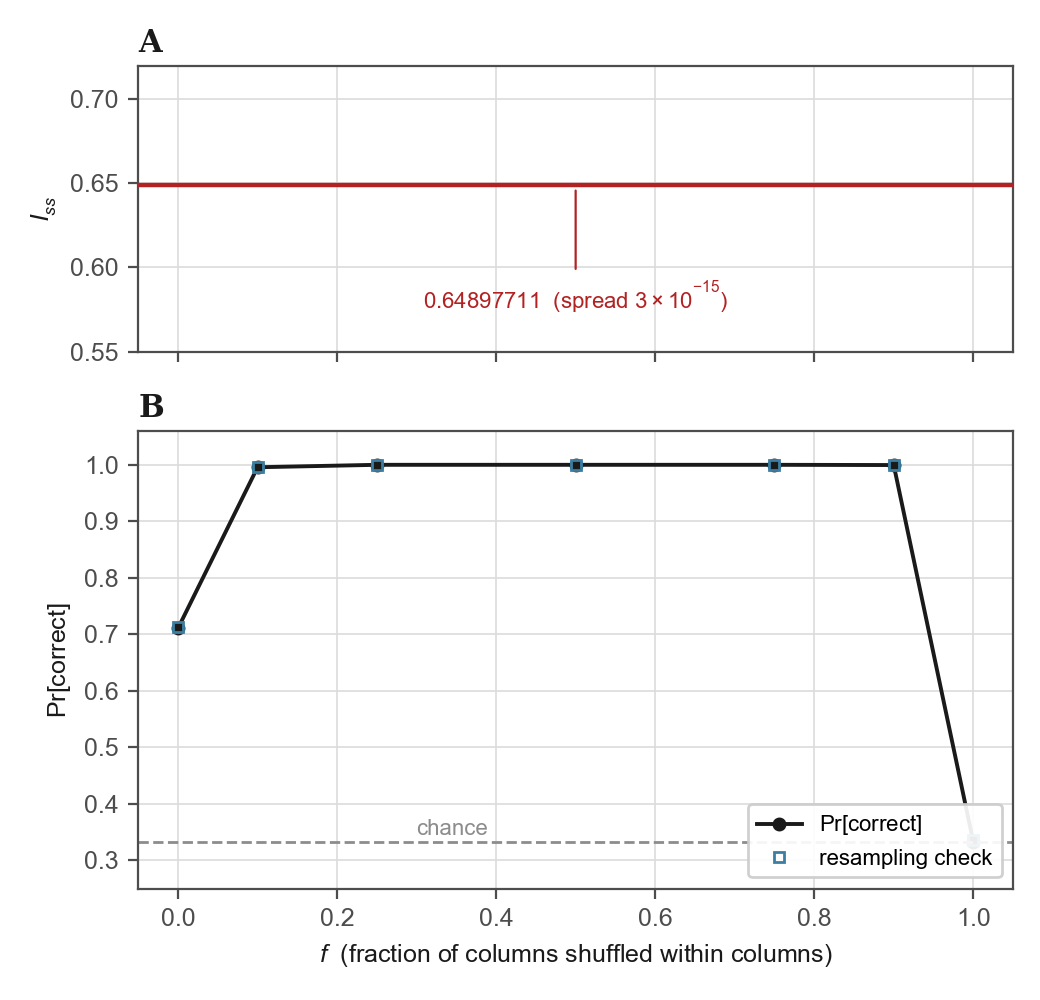
\includegraphics[width=0.75\textwidth]{fig1_iss_flat_power_not}
\caption{$\Iss$ is exactly constant along a family of alignments whose
recovery rate is not. Taxa are permuted within each column, independently per
column, for a fraction $f$ of columns. Panel A: the preservation is exact ---
$\Iss=0.64897711$ at every $f$, spread $3\times10^{-15}$. Panel B: the same
axis, and the recovery rate runs from $0.711$ through $1.000$ to the chance
value $1/3$. Squares are an independent multinomial resampling check on the
mixture distribution.}
\label{fig:flat}
\end{figure}

\begin{figure}[t]
\centering
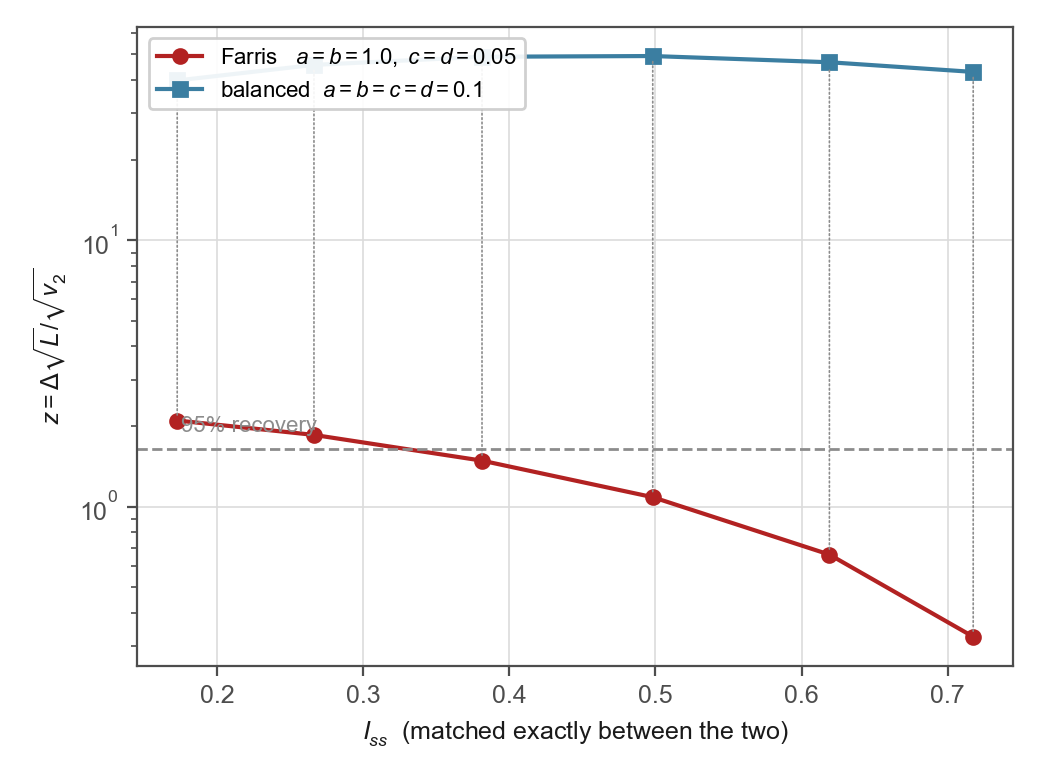
\includegraphics[width=0.75\textwidth]{fig2_matched_iss}
\caption{The same conclusion inside the tree family, without shuffling. For
each $\Iss$ value a Farris tree and a balanced tree are matched exactly on
$\Iss$; both are genuine trees growing under the same model. The standardised
signal differs by factors of $19$ to $125$. At $\Iss=0.1727$ the Farris
tree's internal branch is $0.003$ against the balanced tree's $0.096$.}
\label{fig:matched}
\end{figure}

\begin{figure}[t]
\centering
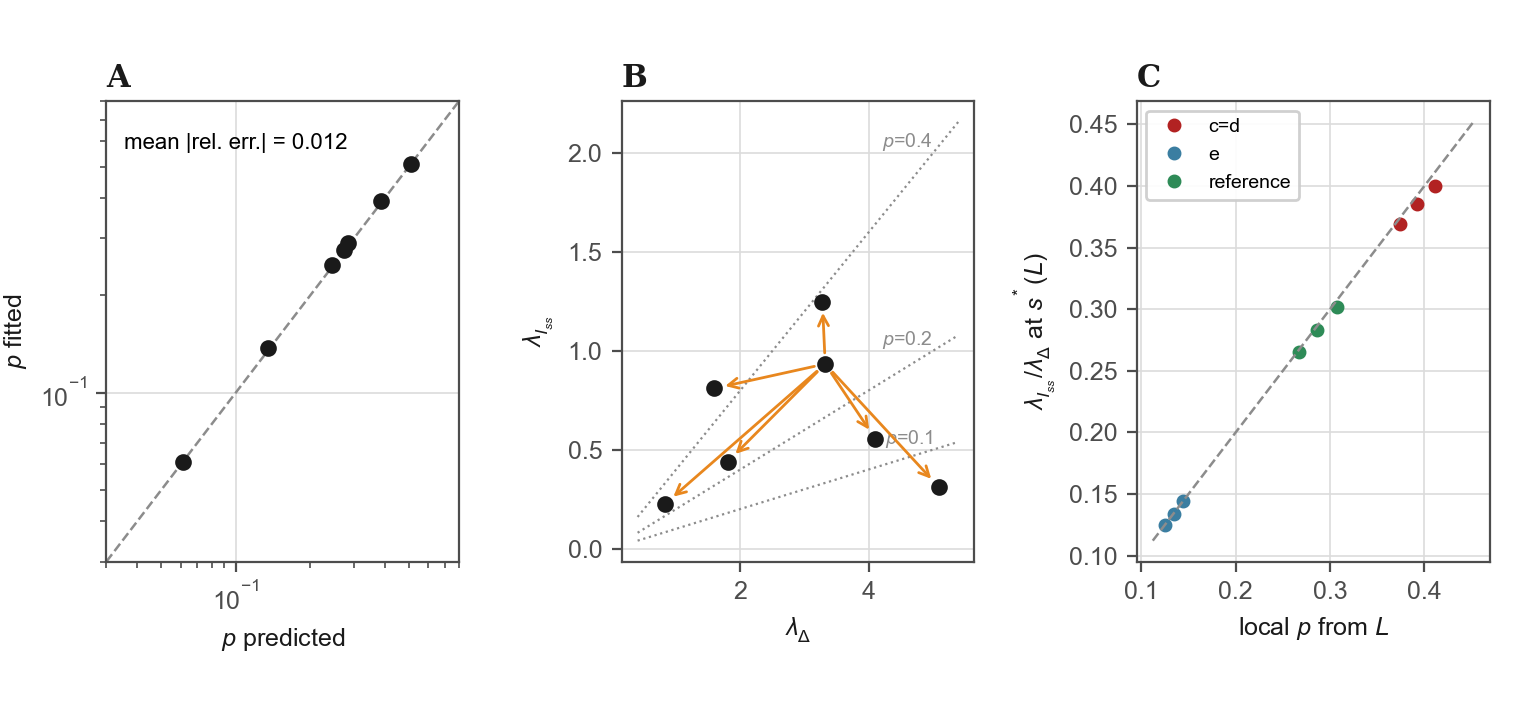
\includegraphics[width=\textwidth]{fig3_exponent_decomposition}
\caption{The exponent is a ratio of two measurable rates. Panel A: predicted
against fitted $p$ over six configurations, on the identity line; mean
absolute relative error $1.4\%$. Panel B: the two rates as a plane, with
iso-$p$ lines; each arrow is one factor changed from the reference. Panel C:
the pointwise comparison, local exponent from $L$ against the locally
measured rate ratio at the critical scale, for three configurations.}
\label{fig:factors}
\end{figure}

\begin{figure}[t]
\centering
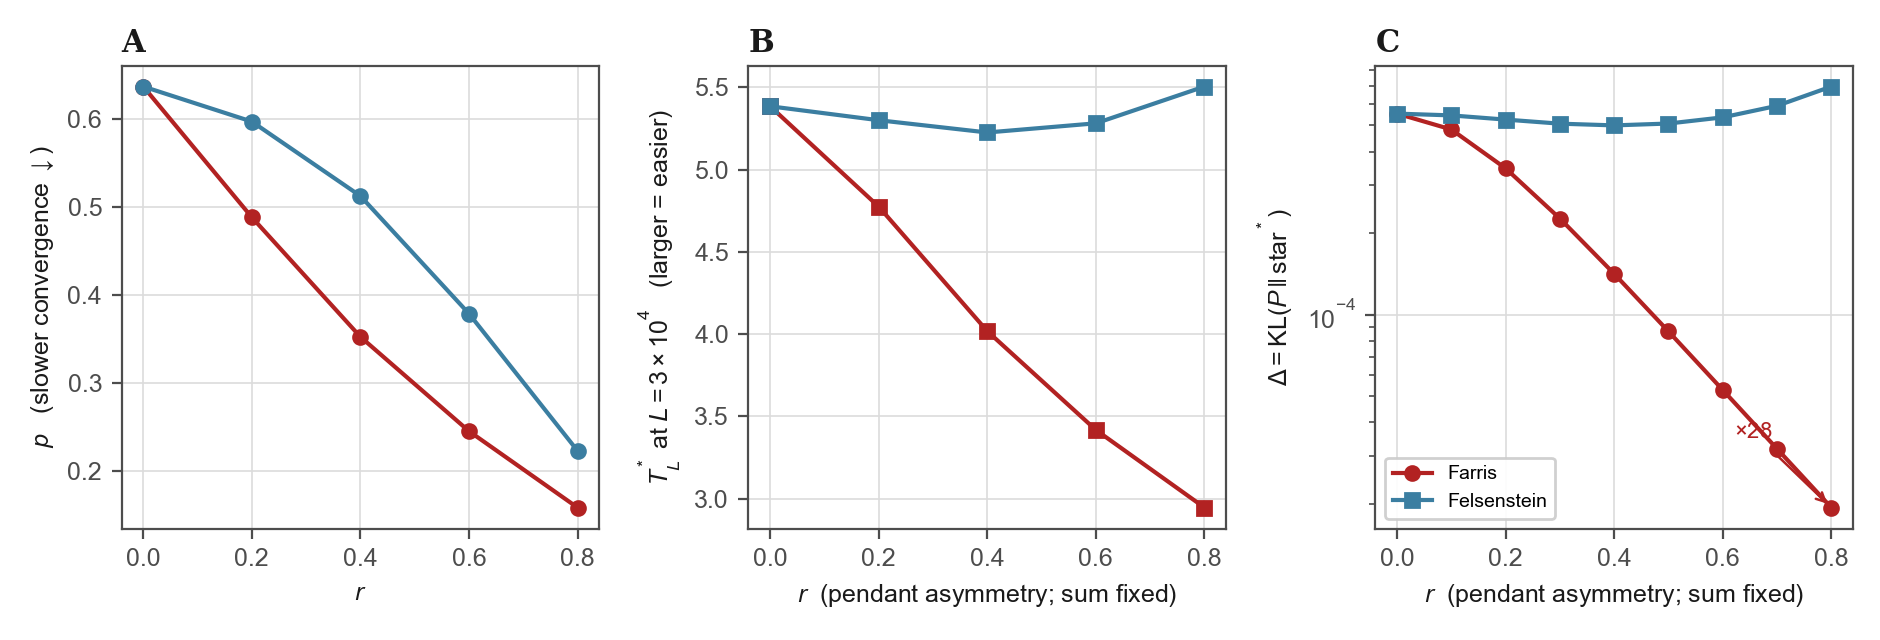
\includegraphics[width=\textwidth]{fig4_arrangement}
\caption{One quantity, three appearances. The pendant sum is fixed at $4$,
the internal branch at $0.2$, and hence the total tree length at $4.2$
throughout; only the arrangement moves. Panel C is the point: $D$ is
exactly the KL distance from the tree to its best star approximation, and the
Farris arrangement drives it down by a factor of $28$ while the Felsenstein
arrangement leaves it flat. That is what the Farris zone is --- the region of
tree space nearest the star. Panels A and B are its two downstream
consequences: the length exponent and the critical tree length. Over the same
range $\Iss$ moves by $2.6\%$.}
\label{fig:arrangement}
\end{figure}

\begin{figure}[t]
\centering
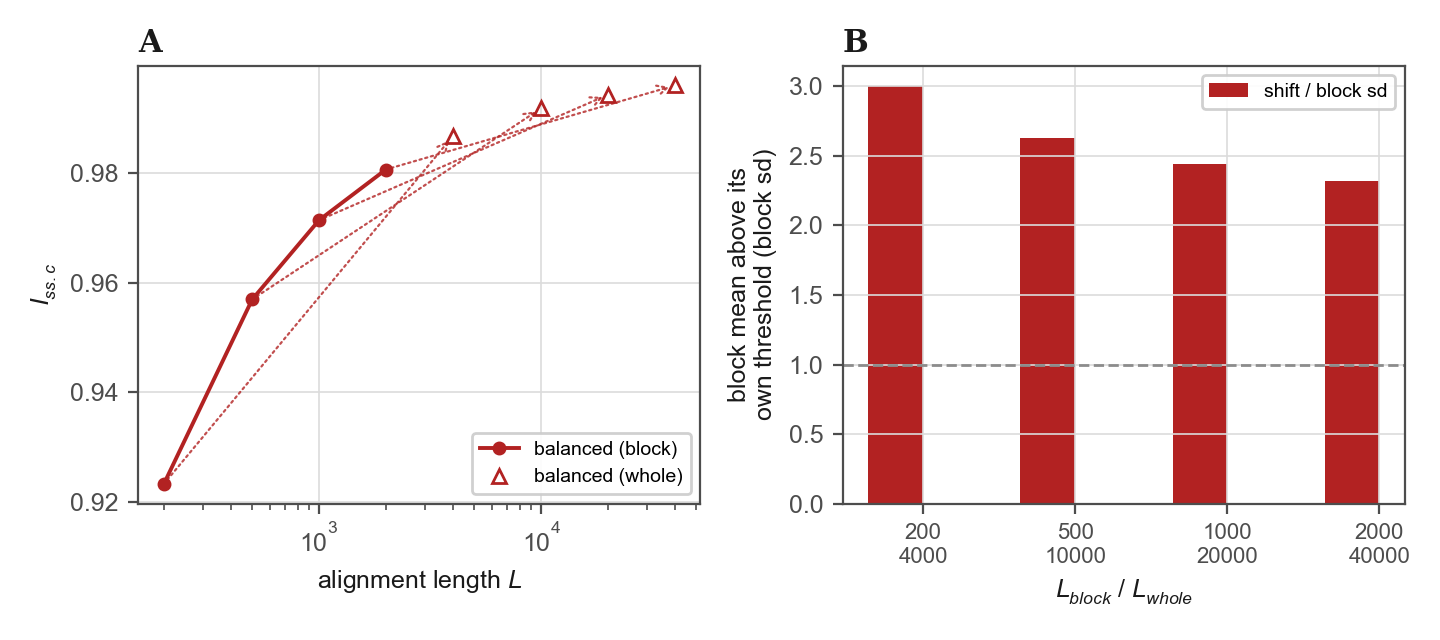
\includegraphics[width=\textwidth]{fig5_domain_and_slicing}
\caption{Where the criterion exists, and what slicing does to it. Panel A:
$\Issc$ against alignment length, with arrows from the block's threshold to
the whole's. Panel B: the block's expected $\Iss$ is the whole's, since the
blocks are slices of the same alignment, whereas the threshold they would be
judged against is the one tabulated for the block's length. The block mean
therefore sits $2.4$ to $3.7$ block standard deviations above its own
threshold, and essentially every block is declared saturated while the whole
passes.}
\label{fig:domain}
\end{figure}

\begin{figure}[t]
\centering
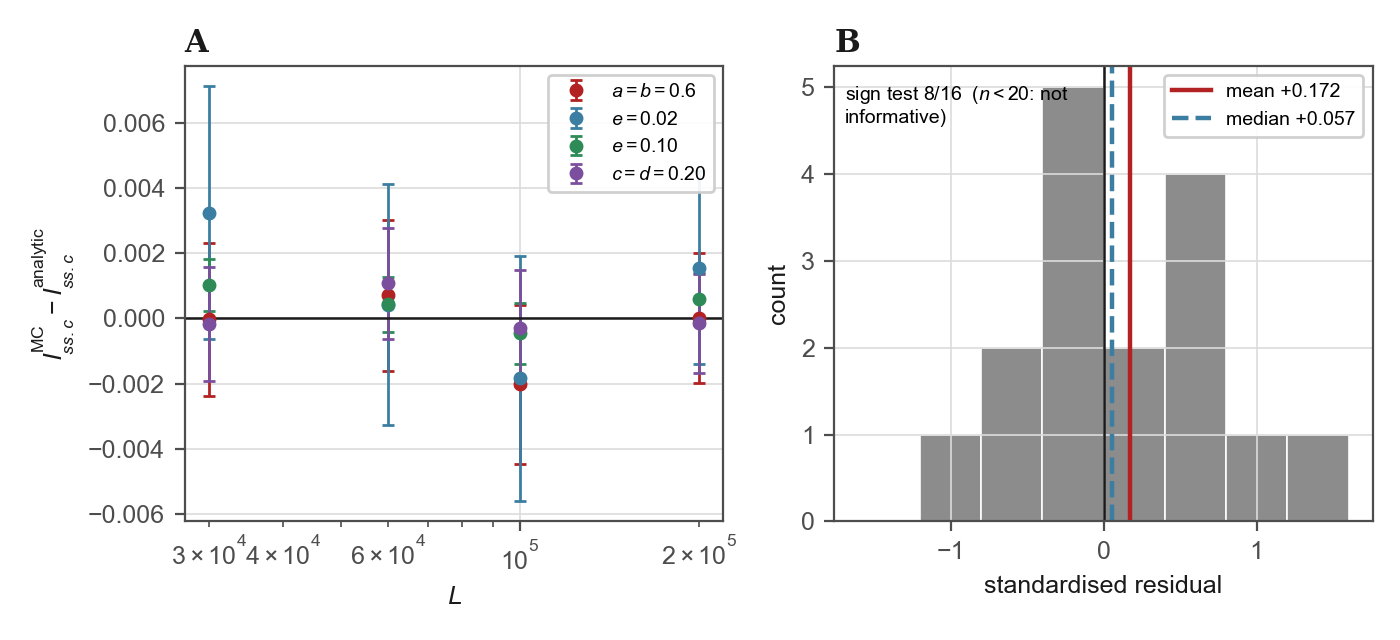
\includegraphics[width=\textwidth]{fig6_validation}
\caption{The analytic chain against our own resampling definition of
$\Issc$, with no external data and no free parameters. Panel A: residuals
with the per-point uncertainty, which varies by an order of magnitude across
the sweep. Panel B: standardised residuals; the mean and median agree to
within their uncertainty and the signs are split. With $16$ points the sign
test has no power, so this is a failure to detect a bias rather than evidence
of none.}
\label{fig:validation}
\end{figure}

\begin{figure}[t]
\centering
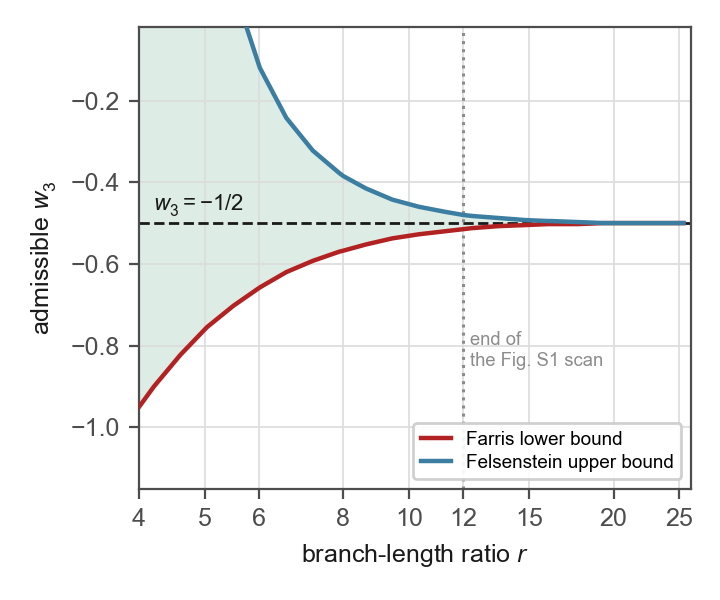
\includegraphics[width=\textwidth]{fig7_w3_window}
\caption{The admissible three-nucleotide weight closes onto $-1/2$. For each
branch-length ratio $r$ --- long branches $0.1r$, short branches $0.1$,
internal $0.1$, the parametrisation of the CASTER supplementary figure S1 ---
two constraints apply: the Farris-zone margin requires $w_3$ above the red
curve and the Felsenstein-zone margin requires it below the blue one. The
admissible set is the shaded region. It is the whole axis for $r<2$, then
closes monotonically from both sides, and by $r\approx19$ it is the single
point $-1/2$. The supplementary scan stops at $r=12$ (dotted line), where the
window is still $0.035$ wide: the last moment before it shuts. $-1/2$ is
therefore not a value that happens to work for both zones but the unique
accumulation point of the admissible set.}
\label{fig:w3}
\end{figure}

\begin{figure}[t]
\centering
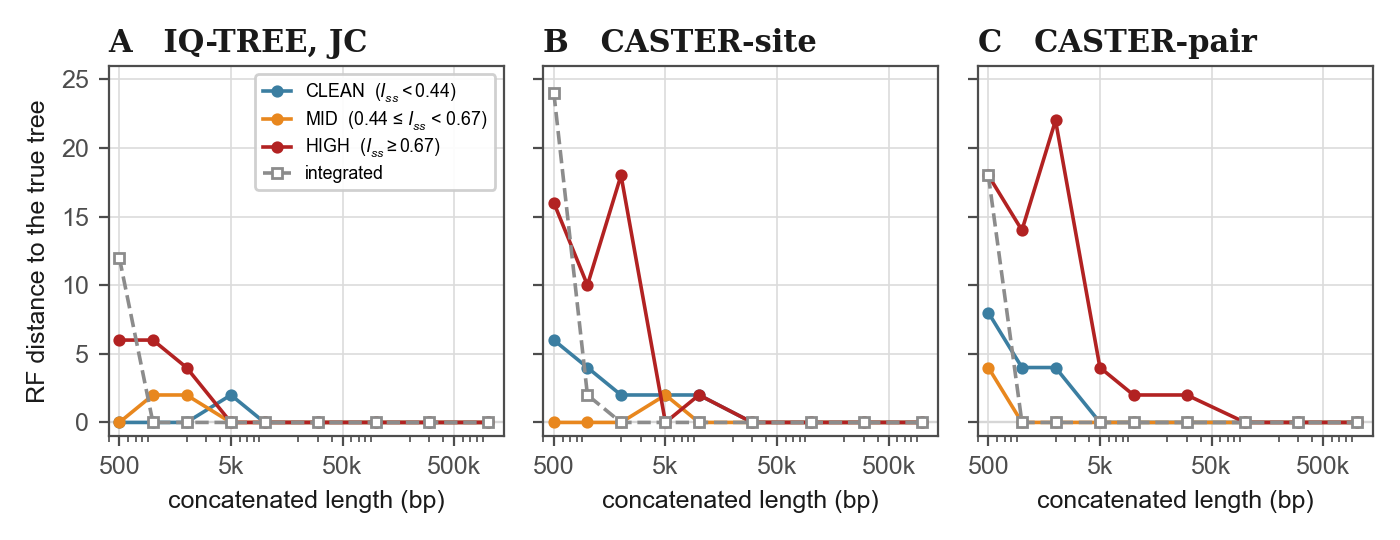
\includegraphics[width=\textwidth]{fig8_band_experiment}
\caption{The band experiment. Fragments are banded by $\Iss$ at the two cuts
measured on the same tree, each arm is truncated to the same $1.025$ Mbp, and
Robinson--Foulds distance to the true tree is plotted against concatenated
length for three methods. HIGH --- the band both calibrations reject --- is
where methods break, and it breaks earlier and harder under CASTER than under
maximum likelihood, which is the price of the weight computed in
Fig.~\ref{fig:w3} paid where there is no long-branch attraction to repair.
MID, the band a $500$ bp calibration rejects and a $10$ kbp calibration
accepts, is indistinguishable from CLEAN and from the integrated arm at every
length above $5$ kbp. From $10$ kbp upward every arm converges to exact
recovery, so at the scale these data are actually analysed the band
composition is not visible in the answer at all. The $500$ bp and $1$ kbp
points are single fragments rather than concatenations and carry no rate.}
\label{fig:bands}
\end{figure}

%% =====================================================================
%% =====================================================================
\subsection{Method notes}
\label{sec:notes}

\paragraph{A fitted branch length is not evidence.} A projection onto the star
is not established by the fitted internal branch being small. Near saturation
the objective is flat along that branch, so an optimiser starting away from
the star stops wherever its gradient runs out, having gained nothing; a small
fitted branch length is a statement about where the optimiser stopped. Judged
by objective instead, no configuration among the $219$ scanned shows a gain
over the star above $2.5\times10^{-6}$.

\paragraph{The degenerate corner.} Permuting to $f=1$ collapses all three
fits onto the same star, so $v_2=v_3=c_{23}\approx0$ and
$\rho=c_{23}/\sqrt{v_2v_3}$ is $0/0$. Clipping $\rho$ to $1$ and taking the
two-way branch returns $\Phi(0)=1/2$ where the answer is $1/3$. The two-way
reduction is valid only when the two \emph{wrong} topologies coincide while
the truth remains distinguishable; when all three coincide it is a genuine
three-way tie. The construction of \S\ref{sec:shuffle} is the only one in the
paper that reaches this corner, which is as it should be: it is the only one
whose purpose is to remove all signal.

\paragraph{Where the maximum-likelihood column comes from.} The
maximum-likelihood entries of \S\ref{sec:genome} are quoted from a full search
with model selection wherever that search and the faster fixed-model search
disagree. Model selection is expensive at the top of the length axis --- on a
$1$ Mbp alignment the model set advanced at roughly one model per minute --- so
it was run on every arm up to $100$ kbp and above that only where the two
searches differ; where they agree, the faster search is reported. ModelFinder
selects JC$+$G4 on every arm on which it was run, which is itself evidence
about the construction: the band matrices concatenate fragments drawn at
scales spanning two orders of magnitude, so the alignment is rate
heterogeneous between fragments and a single-rate fit is misspecified. The
model search finds exactly this, unprompted.

%% =====================================================================

%% =====================================================================
\bibliographystyle{elsarticle-harv}
\bibliography{references}

\end{document}
